\section{Introduction}
% \subsection{Motivation}
Over the decades since its inception, the field of computer science has become increasingly complex and confusing.
This has caused students today to lose track of the picture at large and instead specialize on specific aspects of the field.
Shimon Schocken and Noam Nisam believe that this is an issue and that the best way to understand how computers actually work is to build one from scratch yourself.~\cite[Preface]{nisan2005}

In order to allow students to take this seemingly impossible approach, Schocken and Nisan developed the Nand to Tetris course in 2004, which gives students the opportunity to build an entire computer system themselves.~\cite{1408798}
The system that the participants create over the course of twelve projects is powerful enough to enable the implementation of complex applications and games.\ref{fig:hackenstein-official}

\begin{center}
  \begin{figure}[ht]
    \centering
    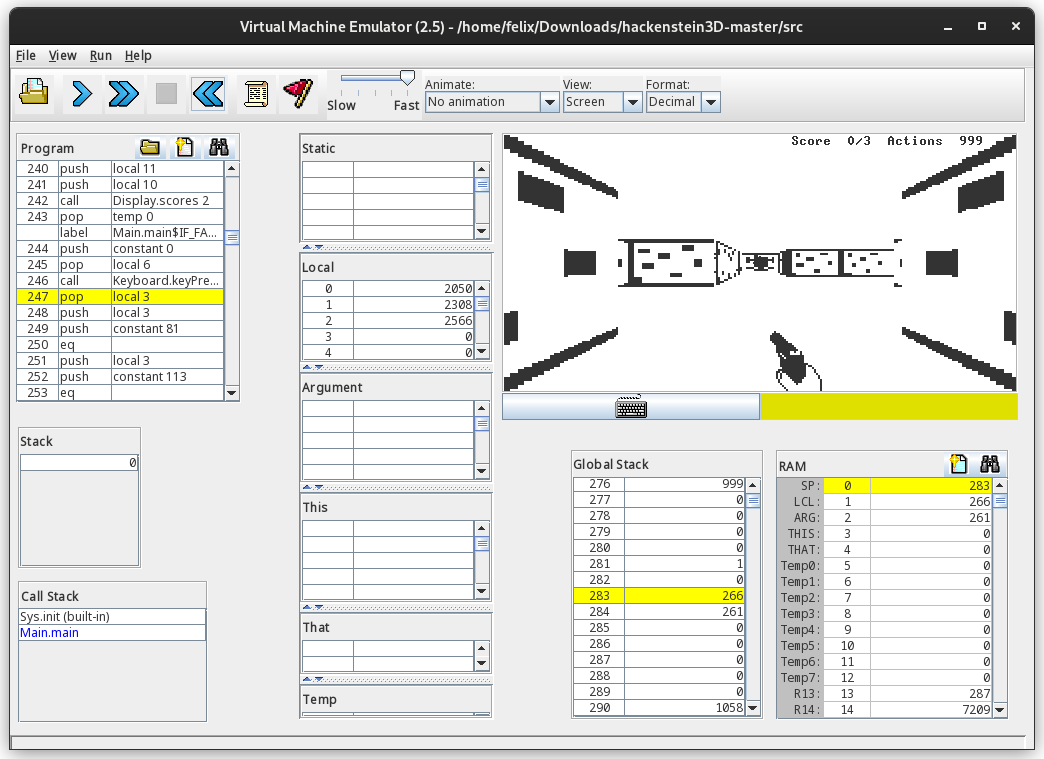
\includegraphics[width=10cm]{fig/hackenstein-official.png}
    \caption{A simple Wolfenstein 3D Clone running in the VM Emulator.}%
    \label{fig:hackenstein-official}
  \end{figure}
\end{center}

To enable students to work on the included projects in a different order than intended, the authors have included a hardware simulator for the initial projects and two different emulators that can simulate the preceding stages of the course.
These emulators are, however, also a frequent point of criticism from course participants, as they increasingly no longer meet the demands of modern users.
Written in Java using the Swing framework, they are not only slow, but also do not adapt to today's higher screen resolutions, making it difficult to actually see the contents of the running application~\ref{fig:hackenstein-official}.
The performance also makes some projects that could otherwise have been implemented on the platform infeasible.
It therefore makes sense to rewrite these emulators to make the course more accessible and thus increase the number of participants.

% \subsection{Contributions}
As part of this work, the two emulators were rewritten as a browser application using WebAssembly. This not only allows support for larger screens and significantly improved performance, but also allows the tools to be used without having to be installed on the student's computer.
The new emulator implementations can now be accessed simply by visiting a URL in a web browser and submitting the bytecode or assembly files via a file selection dialog. Performance has improved significantly, as shown in ~\cref{sec:benchmarks}, allowing users to create even more complex games and applications than before.
In addition, both emulators can be compiled into stand-alone executables that can run the course's test scripts without user input, allowing instructors and course reviewers to use the new emulators to grade submissions.
